\documentclass[12pt, a4paper]{scrartcl}
\usepackage[utf8]{inputenc}
\usepackage[T1]{fontenc}
\usepackage[ngerman]{babel}
\usepackage{SIunits}
\usepackage{csvsimple}
\usepackage{graphicx}
\usepackage{amsmath}
\usepackage{enumitem}
\usepackage{float}
\usepackage{verbatim} %für Kommentare
\usepackage{listings} %Zur Code-Einfügung

\usepackage[
colorlinks,
pdfpagelabels,
bookmarksopen = true,
bookmarksnumbered = true,
linkcolor = black,
plainpages = false,
hypertexnames = false,
citecolor = black
]{hyperref}

%\usepackage{biblatex}
%\addbibresource{Dateien/bibliography.bib}

%\usepackage{titlesec}
%\titleformat{name=\section,numberless}{}
%Entfernt Zahlen vor Kapitelüberschriften
%\titleformat{\chapter}[display]{\normalfont\bfseries}{}{0pt}{\Huge}

\usepackage{tocloft}
%Punktlinie auch nach Kapiteln im Inhaltsverzeichnis
\renewcommand{\cftsecleader}{\cftdotfill{\cftdotsep}}

%Zeilenabstände
\renewcommand{\baselinestretch}{1.5} 

\usepackage{geometry}
%Rand-Abstände
\geometry{verbose, left=20mm, right=20mm, top=30mm, bottom=30mm}

%\usepackage{titlesec}
%\titleformat
%{\chapter} % command
%[hang] % shape
%{\bfseries\Huge} % format
%{\thechapter} % label
%{0.5ex} % sep
%{} % before-code
%[] % after-code


% Für Grafiken
\usepackage{tikz}
\usepackage{pgfplots}
\usetikzlibrary{datavisualization}
\usetikzlibrary{datavisualization.formats.functions}


%%%%%%%%%%%%%%%%%%% Aufteilung: %%%%%%%%%%%%%%%%%%%
% Lea:
%Abstandserkennung
%(GeogebraDatei im doc Ordner)

% Adrian:
%Motoransteuerung
%Umgebung (Räumliche Umgebung des Autos mit Bildern. Auch aus der Sicht des Autos)

% Julian W.:
%Softwareplattform
%Interprozesskommunikation

% Julian F.
%Linienerkennung
%Zielsetzung

% René
%Hardwareplattform
%Einleitung
%Struktur

% Gemeinsam:
%Komplikation und Fehler
%Auswertung


\begin{document}

%%%%%%%%%%%%%%%%%%% STARTSEITE %%%%%%%%%%%%%%%%%%%

\begin{center}
	
	\begin{figure}[H]
		\centering
		
\includegraphics[width=10cm]{Bilder/fh-wedel-logo.png}
	\end{figure}

	\vspace*{1.5cm}
	\Large{\textbf{ R O B O T I K\quad P R A K T I K U M \\ Wintersemester 2017/ 2018\\}}
	\vspace*{1.5cm}
	\huge{\textbf{Dokumentation - Gruppe 1\\}}
	\vspace*{1.5cm}
	
	\vfill
	\begin{table}[h]\centering
		\begin{tabular}{l l}
			 &  tinf101030 - Julian Finck \\
			 & \\
			 & tinf101364 - René P. Keller  \\
			 & \\
			 & inf101301 - Lea Morschel \\
			 & \\
			 & tinf101313 - Adrian Sorge \\
			 & \\
			 & tinf101087 - Julian Weihe \\
		\end{tabular}
	\end{table}

\end{center}


\newpage
\tableofcontents % generiertes Inhaltsverzeichnis
\newpage


%%%%%%%%%%%%%%%%%%% INHALTE %%%%%%%%%%%%%%%%%%%

%%% Neues Kapitel %%%
\section{Einführung}

Das Robotik-Praktikum, wessen Ergebnis diese Dokumentation festhält, fand parallel zur und in Kombination mit der Bachelor-Vorlesung 'Einführung in die Robotik' statt, welche von Herrn Prof. Dr. Ulrich Hoffmann im Wintersemester 2017 gehalten wurde.

Ziel war die Vertiefung und Anwendung der in der Vorlesung vermittelten Inhalte, wobei der diessemestrige Schwerpunkt  auf autonomen Robotern lag. Im Praktikum wurde mit einem AADC\footnote{Audi Autonomous Driving Cup\cite{aadc-website}} 2017 Audi-Modell im Maßstab 1:8 gearbeitet. Es sollte zu Beginn eine nicht näher eingeschränkte Zielsetzung ausgearbeitet werden, welche auf der grundlegenden Anforderung der kollisionsfreien Fahrt aufbauen sollte.

%%% Neues Kapitel %%%
\subsection{Zielsetzung} \label{zielsetzung}

Im Kontext der gegebenen Grundanforderung der Kollisionsvermeidung wurden eigene Ziele definiert. Das Auto sollte später in der Lage sein, einer zentralen blauen Fahrbahnmarkierung zu folgen, dies unter verschiedenen Lichtverhältnissen. Bei Näherkommen eines von Ultraschallsensoren detektierbaren Hindernisses soll das Modell langsamer werden und vor ihm zum Stehen kommen sowie die Fahrt erst wieder aufnehmen, wenn die Sensoren signalisieren, dass die Fahrbahn wieder frei ist.

Die zu Beginn des Praktikums ausgearbeitete Roadmap findet sich in Abbildung \ref{img_Roadmap_Gr1}.
\newpage
Die Umsetzung des Projektes wurde zu Anfang in vier Bereiche unterteilt:
\begin{enumerate}
		\item{Linienerkennung und -verwertung
		\begin{enumerate}
			\item Mittelpunktbestimmung
			\item Testen unter verschiedenen Lichtintensitäten
	\end{enumerate}}
	\item{Abstandserkennung und Kollisionsvermeidung
	\begin{enumerate}
		\item Messwertverarbeitung der Ultraschallsensoren
		\item Messwertglättung durch Filterung (Kalman)
	\end{enumerate}}
	\item {Motorsteuerung
		\begin{enumerate}
		\item Schnittstellendefinition zur Ansteuerung
		\item Steuerung von Geschwindigkeit und Lenkung
		\end{enumerate}}
		\item{Zusammenbringung/ Fusionsschnittstelle
		\begin{enumerate}
			\item Definition und Ausarbeitung des Controllers (Verhaltens-Logik)
			\item Problembehandlung, Feinabstimmung, Testung
		\end{enumerate}}
\end{enumerate}

\begin{figure}
\centering
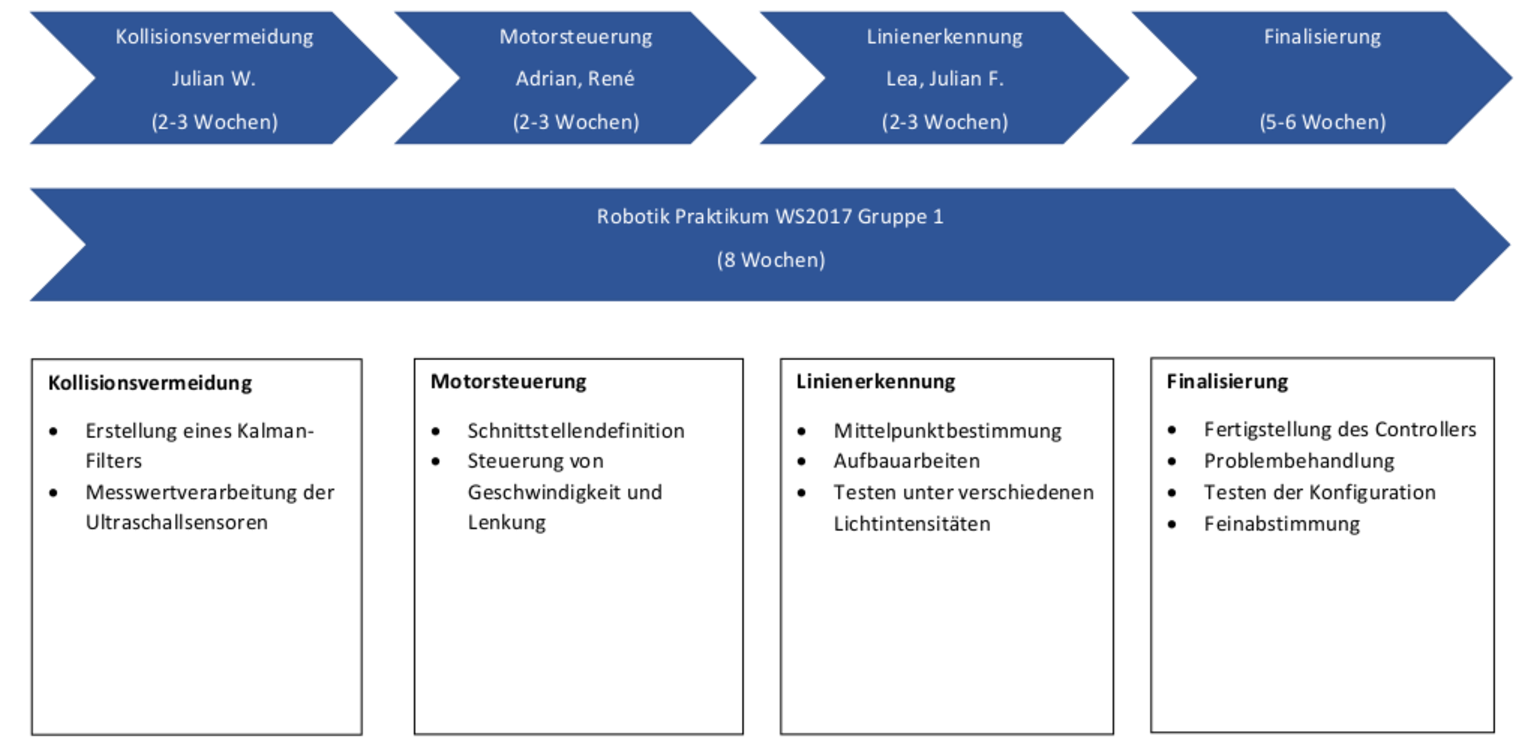
\includegraphics[width=\textwidth, height=8cm, keepaspectratio]{Bilder/Roadmap_Gr1.pdf}
\caption{Zu Projektbeginn erstellte Roadmap}
\label{img:Roadmap_Gr1}
\end{figure}


\newpage
%%% Neues Kapitel %%%
\section{Grundlagen}

Im Folgenden werden die Grundlagen, bestehend aus Aufbau des genutzten Modellautos, der darauf laufenden Software, sowie das genutzte Framework erläutert, welche für das Verständnis des Projektes essenziell sind.

\subsection{Hardwareplattform}

Das Audimodell bietet verschiedene Hardwarekomponenten, um das autonome Fahren zu verwirklichen.

TODO: Bild vom Audi gesamt

\subsubsection{Grundkomponenten}
Die Stromversorgung während der Fahrt wird durch zwei Akkus sichergestellt.

\subsubsection{Rechner}
Herzstück des Audi ist das \emph{GIGABYTE GA-Z170N-WIFI miniITX} Mainboard. Unterstützt wird es von einer \emph{NVIDIA GeForce GTX 1050Ti}. 
TODO: Bild vom Audi, vor allem mit der Intel

\subsubsection{Aktoren}
Angetrieben wird das Modell von vier \emph{Hacker SKALAR 10 21.5 Brushless Motor 1/10}.
Die Lenkung funktioniert über \emph{Absima 'ACS1615SG' Combat Series} Servos. 

\subsubsection{Sensoren}
Die Linienerkennung arbeitet mit der Intelkamera, die mit einer anderen Position und einem anderen Winkel benutzt wird, als im Basismodell. Zum Vergleich siehe Abbild 1 und 2. Grund ist der verbesserte Blick auf den Nahbereich und das mittig ausgerichtete Bild.

TODO: Bild von den Sensoren und Arduinos

Zur Kollisionsvermeidung werden die verbauten Ultrasonic Sensoren verwendet. Ansteuern lassen sich diese über Arduinos, die mit dem Mainboard verbunden sind. Der Audi besitzt insgesamt zehn Stück, von denen fünf, in unterschiedlichen Winkeln, nach vorne, jeweils einer zu jeder Seite und drei, wieder in unterschiedlichen Winkeln, nach hinten ausgerichtet sind. Die drei hinteren Sensoren bekommen nicht so viel Gewichtung, da das Auto in unserem Projekt nicht rückwärts fahren soll.



\subsection{Softwareplattform}
Das Modellauto verwendet die Ubuntu Version 16.04 und zur Bildschirmübertragung ist der x11vcn Serverdienst eingerichtet. Die Software EB Assist ADTF 2.14 von Elektrobit ist installiert, um die damit bereitgestellte Programmoberfläche und das ADTF-Framework \footnote{Automotive Data and Time-Triggered Framework\cite{adtf-website}} zu verwenden.

\subsubsection{ADTF-Framework: Grundlegende Strukturen}
 Das Framework stellt Funktionen zur Kommunikation mit den im Abschnitt 'Hardwareplattform' erläuterten Sensoren und Kameras bereit. Außerdem ermöglicht es eine Programmaufteilung in Funktionsblöcke, \emph{Filter} genannt, welche parallel auf mehreren Prozessorkernen ausgeführt werden können. Die Kommunikation zwischen diesen Blöcken wird über Nachrichtenqueues und Priorisierung vom Framework sichergestellt. Die Ausführung der Funktionsblöcke wird einstellbar periodisch eventgesteuert ausgelöst und beginnt meist mit dem Anstoß zum Auslesen der Sensoren, welche dann das Event über die Queues an andere Funktionsblöcke weitergeben.

Von der Benutzeroberfläche aus lassen sich die Funktionsblöcke grafisch miteinander verbinden, welches die Kommunikation zwischen den Blöcken repräsentiert, und die Ausführung der Funktionen starten. Des Weiteren gewährt die Oberfläche Zugriff auf fertige Funktionsblöcke, etwa zum Anzeigen und Abspeichern von Kamerabildern und Sensordaten oder zum  Abspielen selbiger.
Durch Referenzen aus dem Programm heraus können über die Benutzeroberfläche bestimmte Parameter zur Initialisierung und zur Laufzeit gesetzt werden.


\newpage
%%% Neues Kapitel %%%
\section{Implementierung}

\subsection{Umgebung}

Die Zielsetzung sieht vor, das Auto eine blaue Linie verfolgen zu lassen. Zu Testzwecken wurde daher auf dem Boden eine große, ovalförmige Linienstruktur mit mattblauem Klebeband befestigt, deren Maße etwa 1,5m x 3m beträgt. Zur Vermeidung von störender Spiegelung wurde zudem das Fenster zugestellt, um die Sonneneinstrahlung zu minimieren.

TODO: Bild(er) der Umgebung

\subsection{Projektstruktur}

Das Projektwurde zu Beginn in verschiedene Aufgabenbereiche aufgeteilt, die separat bearbeitet wurden (siehe \autoref{zielsetzung}). Die vier großen Bereiche sind im Folgenden näher beschrieben.

\begin{enumerate}
	\item Linienerkennung und -verfolgung
	\item Abstandserkennung und -verwertung
	\item Motorsteuerung
	\item Fusionsschnittstelle
\end{enumerate}


\subsubsection{Linienerkennung und -verfolgung}
Damit das Auto der blauen Fahrbahnlinie folgen kann, wird die Linie im Kamerabild detektiert. Anschließend wird die Position der Linie ausgewertet um daraus Steuersignale für die Lenkung zu gewinnen. Diese Aufgaben werden von zwei Filtern gelöst:

\paragraph{BlueImgFilter}
Dieser Filter markiert die Fahrbahnlinie und greift dafür auf die OpenCv Bibliothek zurück. Weil die Kamera hauptsächlich den (hellgrauen) Boden unmittelbar vor dem Auto sieht, kann man da-von ausgehen, dass die Fahrbahnlinie im relevanten Suchbereich der einzig blaue Bildinhalt ist.

Zunächst wird das Eingangsbild mit OpenCv vom RGB- in den HSV-Farbraum transformiert, um die Festlegung von Ober- und Untergrenzen für Blauwerte zu vereinfachen. Mittels der OpenCv-Funktion inRange werden anschließend alle nicht blauen Bildinhalte herausgefiltert und ein Binär-bild zurückgegeben, welches alle blauen Flächen markiert. Die endgültigen Farbwertgrenzen erge-ben sich durch Testläufe unter Realbedingungen.    

TODO: Abbildung 1 und 2 (Übernehme ich aus deiner Doku Julian)


\paragraph{OneLineDetect}
Dieser Filter erhält das Binärbild und ermittelt die Position der blauen Linie relativ zur Position des Autos. Dafür wird in einer festgelegten Bildzeile nahe des Unteren Bildrandes nach der größ-ten Anzahl weißer, zusammenhängender Pixel gesucht. Durch die Aufbereitung des Bildes durch den blueImgFilter kann davon ausgegangen werden, dass diese Pixel zur blauen Linie gehören. 

Anschließend wird die Mitte des weißen Pixelabschnittes berechnet und deren Abstand zur Bild-mitte ausgegeben. Dieser Abstand wird auf einen Bereich zwischen -100 und 100 normiert. Über die Filterproperties lässt sich eine Mindestbreite für die Anzahl weißer Pixel festlegen um die De-tektion noch robuster zu gestalten. Sind im aktuell zu bearbeitenden Bild keine oder zu wenig weiße Pixel am Stück, so wird statt einer Zahl zwischen -100 und 100 der Wert -101 ausgegeben.

Für Debugzwecke wird die detektierte Linienmitte mit einem roten Kreis markiert.
Dieser Ansatz setzt voraus, dass das Kameraobjektiv auf der Mittelachse des Modelautos montiert ist.

TODO: Abbildung 3 (übernehme ich genauso)
 

\subsubsection{Abstandserkennung und -verwertung}
Die Abstandserskennung ist eine der wichtigsten grundlegenden Anforderungen an einen autonomen Roboter zur Ermöglichung von gefahrloser Navigation. In diesem Projekt wird sie auf Basis von Messwerten der zehn im Auto verbauten Ultraschallsensoren [TODO: Referenz auf USC-Modell-Bild aus Hardware-Doku-Part] implementiert.

Die eingehenden Abstandswerte liegen im Bereich von 0 bis 400 cm. Diese werden unterschiedlich gewichtet, dann der geringste Anstandswert in eine Geschwindigkeit umgerechnet. Die Übersetzung eines Abstands- in einen Geschwindigkeitswert wurde anhand einer linearen Funktion realisiert, die einen minimalen  Input-Grenzwert zum Anstoßen der Bewegung beinhaltet und gleichsam einen maximalen Input-Wert, ab dem die volle Geschwindigkeit zurück gegeben wird (siehe \autoref{graph_disttospeed}). Dies dient dazu, einen gewissen Mindestabstand beim Fahren nicht zu unterschreiten, sowie zum Ignorieren von Hindernissen, die weiter als ein gewisser Maximalwert von den Sensoren entfernt aufgefasst werden. Letzterer wurde statisch auf 100 cm gesetzt. Im Abstands-Wertebereich von 40 bis 100 gilt somit die lineare Funktion \emph{y = x}.

\begin{figure}[ht]
	\centering
	\begin{tikzpicture}[xscale=0.05,yscale=0.05,domain=0.125:220,samples=400]
		\draw[->] (-10,-10) -- (180,-10) node[below] {$Abstand (\centi\meter)$}; %x-Achse
		\draw[->] (0,-20) -- (0,115) node[left] {$Geschwindigkeit$}; %y-Achse
		\foreach \i in {20,40,...,150} { %x-Achsen-Schritte
			\draw (\i,-9) -- (\i,-11) node[below] {$\i$};
		}
		\foreach \i in {0,10,...,100} { %y-Achsen-Schritte
			\draw (1,\i) -- (-1,\i) node[left] {$\i$};
		}
		\draw[blue] (0,0) -- (40,0) ;
		\draw[blue, dotted] (40,0) -- (40,40);
		\draw[blue] (40,40) -- (100,100) -- (140, 100);
		\end{tikzpicture}
	\caption{Übersetzung von gemessenem Abstand in Geschwindigkeit}
	\label{graph_disttospeed}
\end{figure}

Die statisch festgelegten Mindestabstandswerte für die einzelnen Sensoren führen allerdings zu der unerwünschten Eigenschaft, dass situationsunabhängig die Gewichtung der Sensorwerte konstant bleibt, die vor allem für ein Geradeaus-Fahren mit gewisser Geschwindigkeit optimal ist. Das ist beispielsweise in Kurven problematisch, wo das Hauptaugenmerk nicht mehr geradeaus liegen sollte, da die Geschwindigkeit durch verbeifahrend frontal erkannte Hindernisse unnötig gedrosselt werden würde. Daher wurde eine dynamische Anpassung des relevanten Blickkegels realisiert. Dazu wird über den Parameter des aktuell eingeschlagenen Lenkwinkels jeder Messwert zunächst gemäß einer Gaußkurve gewichtet, bevor der geringste Abstandswert in eine Geschwindigkeit übersetzt wird.
\begin{equation}\label{eq:gaussian-weighted-dist}
weightedSensorVal = 5 - 4 * \exp\Bigl({-3 * 2^{sensorAngle - steeringAngle}}\Bigr)
\end{equation}

\begin{figure}
	\centering
	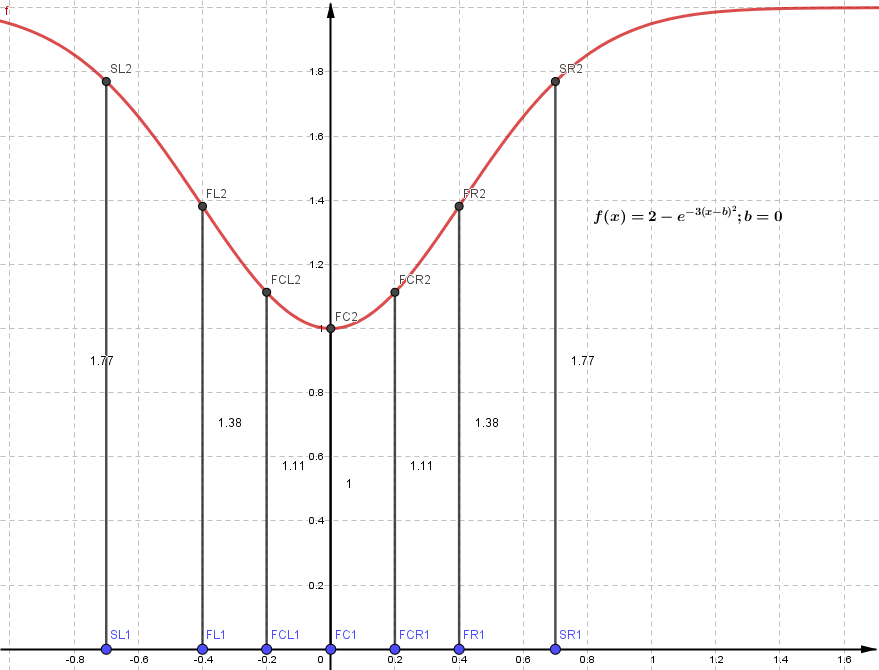
\includegraphics[width=\textwidth, height=8cm, keepaspectratio]{Bilder/Robotik_Gauss_gerade.png}
	\caption{Gewichtung der Abstands-Messwerte beim Geradeaus-Fahren}
	\label{img:gaussian-weighted-dist-straight}
\end{figure}

\begin{figure}
	\centering
	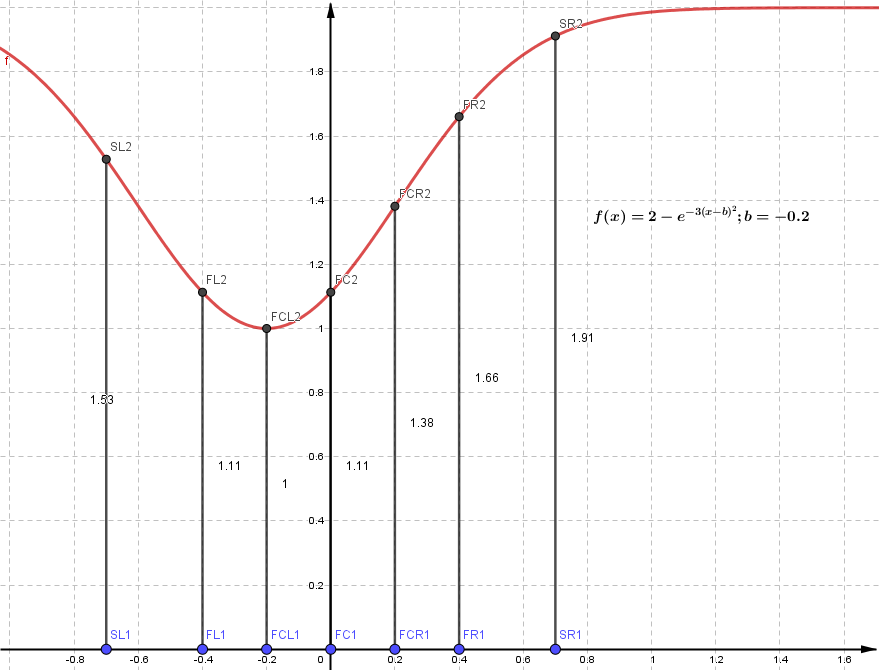
\includegraphics[width=\textwidth, height=8cm, keepaspectratio]{Bilder/Robotik_Gauss_kurve.png}
	\caption{Gewichtung der Abstands-Messwerte beim Kurve-Fahren}
	\label{img:gaussian-weighted-dist-curve}
\end{figure}

Konkret sieht man in Abbildung [x] die fixen Ablesungspunkte der einzelnen Sensoren auf der x-Achse, welche den Sensor-Winkeln in Blickrichtung des Autos angelehnt wurden. Der entsprechende Punkt auf der Gauss-Kurve gibt den jeweiligen Gewichtungs-Faktor an, wobei ein größerer Wert eine größere Unempfindlichkeit bedeutet. Gemäß Lenkwinkel wird nun die Kurve auf der x-Achse verschoben, wodurch die Gewichtung sich auf die entsprechend seitlich liegenden Sensoren verschiebt.


\subsubsection{Motoransteuerung}
Die Hauptaufgaben der Motorsteuerung sind das Reagieren auf Flags, wie beispielsweise das Emergencybreak-Flag, sowie die Motorsteuerungsdaten, welche sie von dem Controller bekommt und an die Arduinokommunication weitersendet.

Wir haben uns entschlossen in diesem Baustein auf Flags zu reagieren, um eine schnellere Reaktion auf kritische Ereignisse, wie zum Beispiel das plötzliche Auftauchen eines Hindernisses zu ermöglichen. Dies erreichen wir, indem wir die Flags direkt aus den Blöcken bekommen, welche die Sensordaten verarbeiten und das Signal nicht erst durch verschiedene Verarbeitungsschritte durchgehen muss. Die Emergencybreak wird erst wieder aufgehoben, sobald ein entsprechendes Signal von den Sensoren kommt.

Außerdem beherscht dieser Baustein als einziger das Protokoll, welches zur Ansteuerung der Motoren mittels der Arduinocommunication verwendet wird. So kann intern ein Protokoll verwendet werden, dass sich deutlich besser lesen und im Falle von Verarbeitungsfehlern debuggen lässt. Da der Motorcontroller eine gewisse Anzahl an Nullen benötigt, um aktiviert zu werden, werden die ersten 150 Geschwindigkeitsdaten auf Null gesetzt. Nach diesen 150 Nullen können dann Geschwindigkeiten an die Motoren gesendet werden. Um eine Geschwindigkeit zu verhindern, die zu schnell für die Ultraschallsensoren ist, haben wir uns entschieden eine maximale Geschwindigkeit festzulegen(momentan 12\%). Sollte ein Wert, der größer als dieser ist, an die Motorsteuerung gesendet werden, so wird dieser ignoriert und ein Fehler in der Konsole ausgegeben.

\paragraph{Umgebung}
Das Auto wurde programmiert, um eine blaue Linie zu verfolgen. Es wurde ein großes blaues Oval auf den Boden geklebt. Das verwendete Klebeband ist recht Matt, um Spiegelungen zu vermeiden, jedoch wurde in der Testung die Sonneneinstrahlung minimiert.


\subsubsection{Fusionsschnittstelle}
Interprozesskommunikation

Da die Programmierung in verschiedenen Funktionsblöcken erfolgte, musste eine einheitliche Kommunikation sichergestellt werden. Hierzu wurde eine separate Funktionssammlung erstellt, die von allen Funktionsblöcken inkludiert wurde. Sie beinhaltet Definitionen über den Nachrichtentyp und die Zusammensetzung strukturierter Datentypen. Da der vom ADTF gestellte Ablauf zum Senden oder Empfangen eines bestimmten Nachrichtentyps zur Codeverdopplung in den Funktionsblöcken führen würde, wurden die Funktionen zusammengefasst und ausgelagert. Damit ließ sich auch einheitlich sicherstellen, dass Funktionsblöcke beim Empfangen die Nachricht erst Kopierten, bevor deren Inhalt verändert wurde.

\subsection{Fallstricke: Komplikationen und Fehler}


\newpage
%%% Neues Kapitel %%%
\section{Auswertung}


\begin{comment}
\newpage
%%% Neues Kapitel %%%
\section{Literaturverzeichnis}

\begin{enumerate}
	\item Im$^2$C Geschichte,  https://www.i2c-bus.org/twi-bus/
	\item Das Im$^2$C-Bus-System
	\item http://www.g-heinrichs.de/pdv/i2c.pdf
	\item http://www.robot-electronics.co.uk/i2c-tutorial
	\item http://www.atmel.com/Images/8183S.pdf
\end{enumerate}
\end{comment}


\newpage
\addcontentsline{toc}{section}{Abbildungsverzeichnis}
\listoffigures

\newpage
\begin{thebibliography}{9}
	\bibitem{aadc-website}
	\textit{AADC-Website},
	Audi AG:
	\url{https://www.audi-autonomous-driving-cup.com/wettbewerb/ueberblick/}
	
	\bibitem{adtf-website}
	\textit{ADTF-Website},
	Elektrobit:
	\url{https://www.elektrobit.com/products/eb-assist/adtf/}
	
	\bibitem{im2c-geschichte}
	\textit{Im$^2$C-Geschichte}
	\url{https://www.i2c-bus.org/twi-bus/}
	
	\bibitem{im2c-bussystem-ehi}
	E. Eube, G. Heinrichs, U. Ihlefeldt,
	\textit{Im$^2$C-Bussytem},
	Fortbildungsveranstaltung in Mönchengladbach, 23.08.2008:
	\url{http://www.g-heinrichs.de/pdv/i2c.pdf}
	
	\bibitem{im2c-bussystem-robotelectronics}
	\textit{Im$^2$C-Bussytem},
	Robot Electronics:
	\url{http://www.robot-electronics.co.uk/i2c-tutorial}

\end{thebibliography}

\begin{comment}
\newpage
%\nocite{*}
\cite{aadc-website}
\cite{im2c-bussystem}
\cite{im2c-geschichte}
\addcontentsline{toc}{section}{Literaturverzeichnis}
\bibliography{Dateien/bibliography}
\bibliographystyle{ieeetr}
%\printbibliography
\end{comment}


\begin{comment}
\newpage
\addcontentsline{toc}{section}{Tabellenverzeichnis}
\listoftables

\newpage
\addcontentsline{toc}{section}{Listings-Verzeichnis}
\renewcommand\lstlistlistingname{Listings-Verzeichnis (Quellcode)}
\lstlistoflistings
\end{comment}


\end{document}
